
\documentclass[runningheads,a4paper]{llncs}

\usepackage{amssymb}
\setcounter{tocdepth}{3}
\usepackage{graphicx}
\usepackage{amsmath}


\usepackage{url}
\urldef{\mailsa}\path|chit8942@vandals.uidaho.edu|

\newcommand{\keywords}[1]{\par\addvspace\baselineskip
\noindent\keywordname\enspace\ignorespaces#1}

\begin{document}

\mainmatter  % start of an individual contribution

\title{CS520 Semester Project 2015 \\ DSRC Reliability during Congestion in Intelligent Transportation System}

\titlerunning{DSRC Reliability}


\author{
Anup Chitraker
\and
Chihsiang Wang\\
}
%
\authorrunning{DSRC Reliability}

\institute{Department of Computer Science\\ University of Idaho\\
Moscow, Idaho 83843\\
\mailsa\\}

\maketitle


\begin{abstract}
In VANET (Vehicular Ad-hoc Network), vehicles equipped with short range radios communicate with each other (Vehicle-to-Vehicle - V2V) and with the  road side infrastructure (Vehicle-to-Infrastructure - V2I) to enable range of applications from internet access and driver assistance to transportation safety and emergency response. Network topology in VANET changes frequently due to high node mobility. V2V and V2I operates in the 75 MHz Dedicated Short Range Communication (DSRC) spectrum. The spectrum is allocated within 5.85 - 5.925 GHz band which is divided into one control channel and six service channels.
\\
\\
All vehicles will broadcast their state information such as location, speed, vehicle size, etc., frequently in Basic Safety Message (BSMs). According to the standards, each vehicle should transmit one BSM every 100 milliseconds in DSRC. When many vehicles compete for the media access, the channel capacity might not handle the flood of BSMs thereby reducing the reliability of system.
\\
\\
This paper summarizes ongoing research on identifying possible solutions that deals with congestion specially on VANET and how they addressed the reliability issues of the communication.

\keywords{Congestion Control, VANET, Bandwidth Efficiency, Power Control, Node Density, Redundancy, DSRC}
\end{abstract}

\section{Introduction}
\begin{enumerate}
	\item How Reliability of DSRC is presented in literature?
	\item Show the reliability of DSRC with increasing distance.
	\item Show the effect of power and channel switching in the reliability of the DSRC
		\subitem Power modulation won't work (from experimental data we have). 
		\subitem Channel switching somehow increases the reliability however it does not seem to work during congestion - consumes more bandwidth (since we have limited bandwidth).
	\item Solution could be to review the MAC layer.
		\subitem review some congestion control algorithm and see if they might help increasing the reliability of the DSRC.
	
\end{enumerate}
Quality of Service is one of the main concerns in any type of wireless communication. In high density environment, each vehicle broadcasts message flood at a high frequency, that can easily congest the CCH channel. Keeping CCH channel free from congestion is very important in order to ensure timely and reliable delivery of BSMs.

\subsection{DSRC}

\begin{enumerate}
	\item[Note:] Channels, bandwidth, standards..
\end{enumerate}
In U.S. Federal Communications Commission (FCC) has allocated 75 MHz DSRC spectrum in the 5.9 GHz band. The spectrum consists of one control channel (CCH) and six service channels (SCHs) to be used by Intelligent Transportation Systems (ITS) as shown in Figure~\ref{Fig-Channels}.

%-------------begin plots -----
\begin{figure}[thpb] 
	\centering
	\includegraphics[width=5.5in]{Fig-Channel-power.png}
	\caption{DSRC channels and Power Limit \cite{IEEE-2003}}
	\label{Fig-Channels}
\end{figure}
%-------------end plots -----
\subsection{Current DSRC Challenges}
\begin{enumerate}
	\item[Note:] BSM failure, Mutipath delay spread, Doppler spread
\end{enumerate}

\subsubsection{PHY Layer}
Vehicular communications occur in a challenging environment involving fast moving vehicles and a wide range of obstacles that can degrade radio performance such as buildings, surrounding bigger vehicles, intersections, tunnels, bridges, surrounding bigger vehicles, intersections, tunnels, bridges.\cite{IEEE-2007}
\begin{enumerate}
\item Muti-path Delay Spread

\item Mobility
\end{enumerate}

In summary, the vehicular communication channel can be highly frequency selective – due to multipath delay spread, and highly time selective – due to vehicle mobility. It can be easily estimated that the 50\% coherence bandwidth in some scenarios is roughly in the order of ∼1MHz and 50\% coherence time can be as short as ∼0.2ms. This leads to two challenges of adapting the traditional IEEE 802.11 solution to vehicular communications.\cite{IEEE2013}
\begin{enumerate}
\item Channel estimation error in vehicular environment due to time-selective and frequency selective fading;
\item Lack of time-interleaving in fast time-selective fading channels.
\end{enumerate}

\begin{figure}[thpb] 
	\centering
	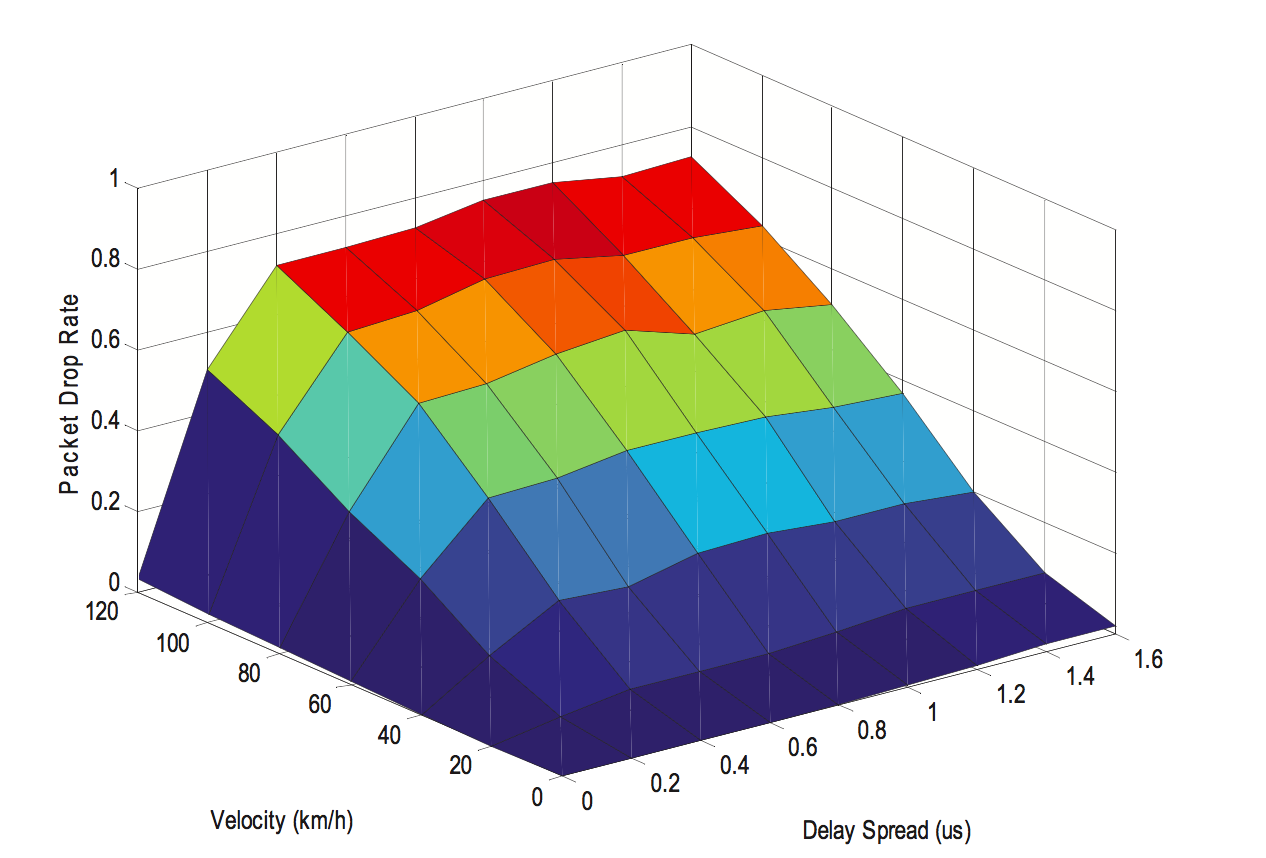
\includegraphics[width=3.5in]{V and DS.png}
	\caption{Conventional IEEE 802.11a implementation \cite{IEEE2013}}
	\label{Fig-Channels}
\end{figure}

\subsubsection{MAC Layer}









\subsection{MAC Protocol in DSRC}

\section{Related Work}

\begin{enumerate}
	\item Describe related work on channel redundancy and message dissimilarity.
	
	\item Many paper claims increasing data rate might increase performance however our experiment may present counter to their literature.
	
	\item Data collected from Experimental Setup:
		%-------------begin plots -----
		\begin{figure}[thpb] 
			\centering
			\includegraphics[width=4.0in]{pdr-3-vs-6-Mbps.png}
			\caption{Reliability of DSRC communication over various data transmit rate}
			\label{Fig-Pdr}
		\end{figure}
	%-------------end plots -----
	\item Specifications:
		\subitem 10 BSM per second
		\subitem Data Transmit Rate: 3Mbps and 6Mbps
		\subitem Transmit Power: 18 dBm
		\subitem Channel 172
		\subitem Continuous Mode
	
	\item Result:
		\subitem Increase in BSM transmit rate; Compete for media access; Decrease in Reliability
\end{enumerate}





%\section{Reliability and Redundancy}
%\begin{enumerate}
%	\item Define reliability in the context of DSRC Safety Applications and set stage for product rule (explain here) of unreliabilities.
%	\item Suggest (as in related work) to increase redundancy levels of messages. Two options:
%		\subitem  Stay on channel or use different channels. Bring in argument of power.  
%		\subitem So question: given a channel (high or lower power) what are the improvements if the rate of BSM of individual vehicles increases. Use figure to show redundancy configurations.
%\end{enumerate}

\section{Analysis of MAC Layer Performance}
\begin{enumerate}
	\item Investigate the impact of increasing BSM rates: 
	\subitem Show model for calculating PDR impact of collisions in unjammed environment, i.e., simply based on message density (vehicle density).
	\item Introduce "Figure direct" and argue how normal, 2x and 3x approaches affect 90\% PDR requirement from Standard.
	\item The case of the hidden nodes is significantly worse. (Include or not?)
\end{enumerate}

\section{Conclusions}



%\section{Introduction}
%\begin{enumerate}
%	\item Introduce ITS and connected vehicles
%	\item Connected Vehicle use DSRC communications: explain WAVE and DSRC and channels. Show table of channels with powers from previous papers
%	\item Introduce safety applications FCW, EEBL, DNPW and BSW+LCW. and the concept of BSM.
%	\item Explain that they work of they relate to parallel RBD, e.g., they fail if no messages arrive during critical time periods.  Use FCW as example
%	\item Explain MAC layer of 802.11p
%\end{enumerate}
%\subsection{DSRC/WAVE}
%\subsection{MAC Layer in 802.11p}
%
%\section{Analysis of 802.11p MAC Layer Performance}


\begin{thebibliography}{4}
	\bibitem{FINA2014}
	 A. Serageldin, and A. Krings, {\em The Impact of Dissimilarity and Redundancy on the Reliability of DSRC Safety Applications}, Proc. Tenth International Symposium on Frontiers of Information Systems and Network Applications, (FINA 2014), Victoria, Canada, May 13-16, 2014.
	
	\bibitem{NIMS2014}
	A. Serageldin, and A. Krings, {\em The Impact of Redundancy on DSRC Safety Application Reliability under Different Data Rates}, Proc. 6th International Conference on New Technologies, Mobility and Security, (NTMS 2014), Dubai, March 30 - April 2, 2014.
	
	\bibitem{IEEE2013}
	X. Wu, S. Subramanian{\em Vehicular Communications Using DSRC: Challenges, Enhancements, and Evolution}, IEEE J. Sel. Areas Commun., vol. 31, no. 9, pp. 399-408, Sep., 2013
	
	\bibitem{SEPT2010}
	Y.P. Fallah, C.L. Huang, R. Sengupta, and H. Krishnan, {\em Congestion Control Based on Channel Occupancy in	Vehicular Broadcast Networks}, IEEE Vehicular Technology Conference (VTC-Fall), September 2010. 
	
	\bibitem{ICC2010}
	F. Ye, R. Yim, J. Zhang, and S. Roy, {\em Congestion Control to Achieve Optimal Broadcast Efficiency in VANETs}, Communications (ICC),
	2010 IEEE International Conference on, 2010, pp. 1–5.
	
	\bibitem{FCC2004}
	{\em Amendment of the Commission's Rules Regarding Dedicated Short-Range Communication Services in the 5.850-5.925 GHz Band (5.9 GHz Band)}, Federal Communications Commission FCC 03-324, 2004.
	
	\bibitem{IFIP2008}
	M.S.Bouassida and M.Shawky, {\em On the congestion control within vanet}, Wireless days,2008. WD '08 1st IFIP Digital Object Identifier: 10.1109/WD.2008.4812915 Publication Year: 2008 , Page(s): 1 – 5
	
	\bibitem{F-69621}
	R. Stanica, E. Chaput, A. Beylot, {\em Reverse back-off mechanism for safety vehicular ad hoc networks}, Université de Lyon, INSA Lyon, CITI-INRIA UrbaNet, F-69621, Villeurbanne, France.
	
	\bibitem{IEEE-2012}
	X. Yin, X. Ma, and K. S. Trivedi, {\em An Interacting Stochastic Models Approach for the Performance Evaluation of DSRC Vehicular Safety Communication}, IEEE Trans. on Computers, accepted, 2012.	
	
	\bibitem{WLAN2011}
	{\em Adaptive Congestion Control of DSRC Vehicle
	Networks for Collaborative Road Safety
	Applications}, IEEE International workshop on Wireless Local Networks, 2011 
	
	\bibitem{ICC2001}
	S.J. Lee and M. Gerla, {\em Dynamic Load-Aware Routing in Ad hoc Networks}, Proceedings of ICC 2001.
	
	\bibitem{VTC2008}
	Z. Y. Rawshdeh and S. M. Mahmud, {\em Media Access Technique for Cluster-Based Vehicular
	Ad Hoc Networks}, IEEE 68th Vehicular Technology Conference Fall (VTC 2008-Fall). September 2008 
	
	\bibitem{ACM2006}
	N. Balan and J. Guo, {\em Increasing Broadcast Reliability in Vehicular Ad Hoc Networks}, Proc. 3rd ACM Int. Workshop VANET, ACM MobiCom,  pp.104 -105 2006
	
	\bibitem{IEEE2005}
	Xin, W., Kar, K., {\em Throughput Modelling and Fairness Issues in CSMA/CA Based Ad-Hoc Networks}, 24th Annual Joint Conference of the IEEE Computer and Communications Societies (2005)
	
	\bibitem{INFOCOM2010}
	P. Li, Y. Fang, and J. Li, {\em Throughput, Delay, and Mobility in Wireless Ad Hoc Networks}, INFOCOM, 2010.
	
	\bibitem{SECON2004}
	R. M. de Moraes, H. R. Sadjadpour, and J. Garcia-Luna-Aceves, {\em Throughput-Delay Analysis of Mobile Ad-hoc Networks with a Multi-Copy Relaying Strategy}, SECON, 2004.
	
	\bibitem{IEEE-2003}
	J. Zhu and S. Roy, {\em MAC for Dedicated Short Range Communications in Intelligent Transport Systems}, IEEE Commun. Mag.,  vol. 41,  no. 12,  2003

	\bibitem{IEEE-2007}
	Cheng, et. al., {\em obile vehicle-to-vehicle narrow-band channel mea- surement and characterization of the 5.9GHz DSRC frequency band}, IEEE J. Sel. Areas Commun., Oct. 2007.

	\bibitem{Berkeley-2008} 
	I. Tan, et. al., {\em Measurement and analysis of wireless channel impair- ments in DSRC vehicular communications}, Tech. Rep., UC Berkeley, Apr. 2008.

	\bibitem{IEEE-2009} 
	S. Sai, et. al., {\em Field evaluation of UHF radio propagation for an ITS safety system in an urban environment}, IEEE Commun. Mag., 2009.

	
%	--------- VERIFY THIS ONE
%		\item "Start-to-Destination Driving Route Reservation (S2D-DRS)"\\Source: Vehicular Communication Networks: Challenges, Solutions, and Services
%	\item
%	Booysen, M.J.; Zeadally, S.; van Rooyen, G.-J., {\em Survey of MAC Protocols for Vehicular Ad Hoc Networks}, Communications, IET, vol.5, no.11, pp.1619-1631, July 22 2011. 
	
	

%\bibitem{SAEJ2735}
%{\em Dedicated Short Range Communications (DSRC) Message Set Dictionary. Society of Automotive Engineers}, SAE J2735, November 2009.
%
%\bibitem{IEEE802.11p}
%{\em IEEE Standard for Information technology--Telecommunications and information exchange between systems--Local and metropolitan area networks--Specific requirements Part 11: Wireless LAN Medium Access Control (MAC) and Physical Layer (PHY) Specifications Amendment 6: Wireless Access in Vehicular Environments}, IEEE Std 802.11p, 2010.
%
%\bibitem{IEEE802.11}
%IEEE 802.11, Part 11: Wireless LAN Medium Access Control (MAC) and Physical Layer (PHY) Specifications, IEEE Std., June 2007.
%

%
%\bibitem{Serageldin2014}
%A. Serageldin, and A. Krings, {\em The Impact of Redundancy on DSRC Safety Application Reliability under Different Data Rates}, Proc. 6th International Conference on New Technologies, Mobility and Security, (NTMS 2014), Dubai, March 30 - April 2, 2014.
%
%\bibitem{Hassan2011}
%Hassan, M.I.; Vu, H.L.; Sakurai, T., {\em Performance Analysis of the IEEE 802.11 MAC Protocol for DSRC Safety Applications}, Vehicular Technology, IEEE Transactions on , vol.60, no.8, pp.3882,3896, Oct. 2011.
%
%\bibitem{VSCA2011}
%Vehical Safety Communications-Applications (VSC-A) Final Report. DOT HS 811 492 A. U.S. Department of Transportation, NHTSA. September 2011.

\end{thebibliography}

\end{document}
